\appendix

\chapter{图表与公式}

\subcaptionsetup[figure]{skip=0pt}

\begin{figure}[ht]
  \vspace*{-1.2cm}
  \centering
  \subcaptionbox{$      L_{-1}$}{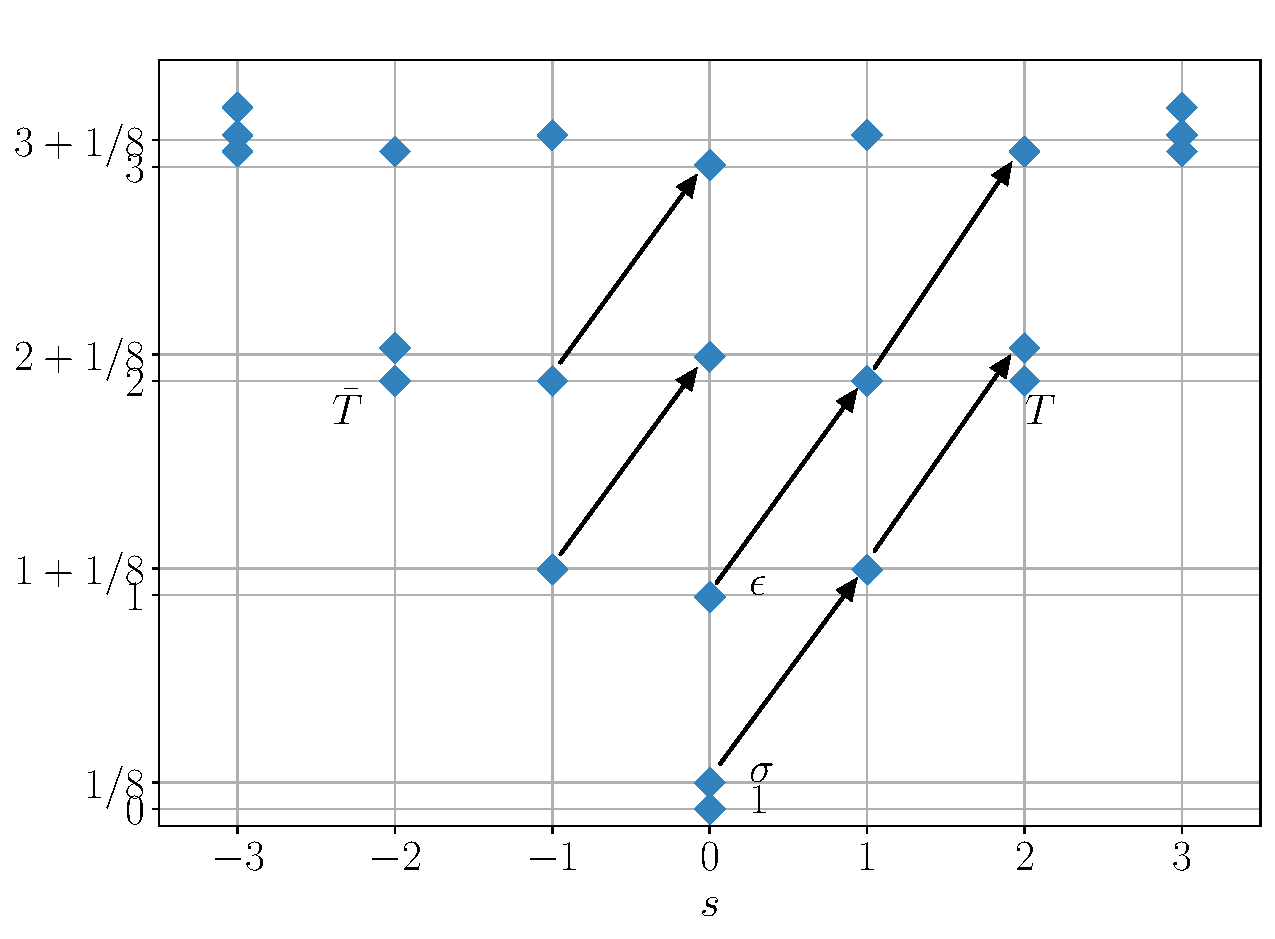
\includegraphics[width=0.42\textwidth]{images/virasoro/ising-lm1.pdf}}    \qquad
  \subcaptionbox{$\bar{L}_{-1}$}{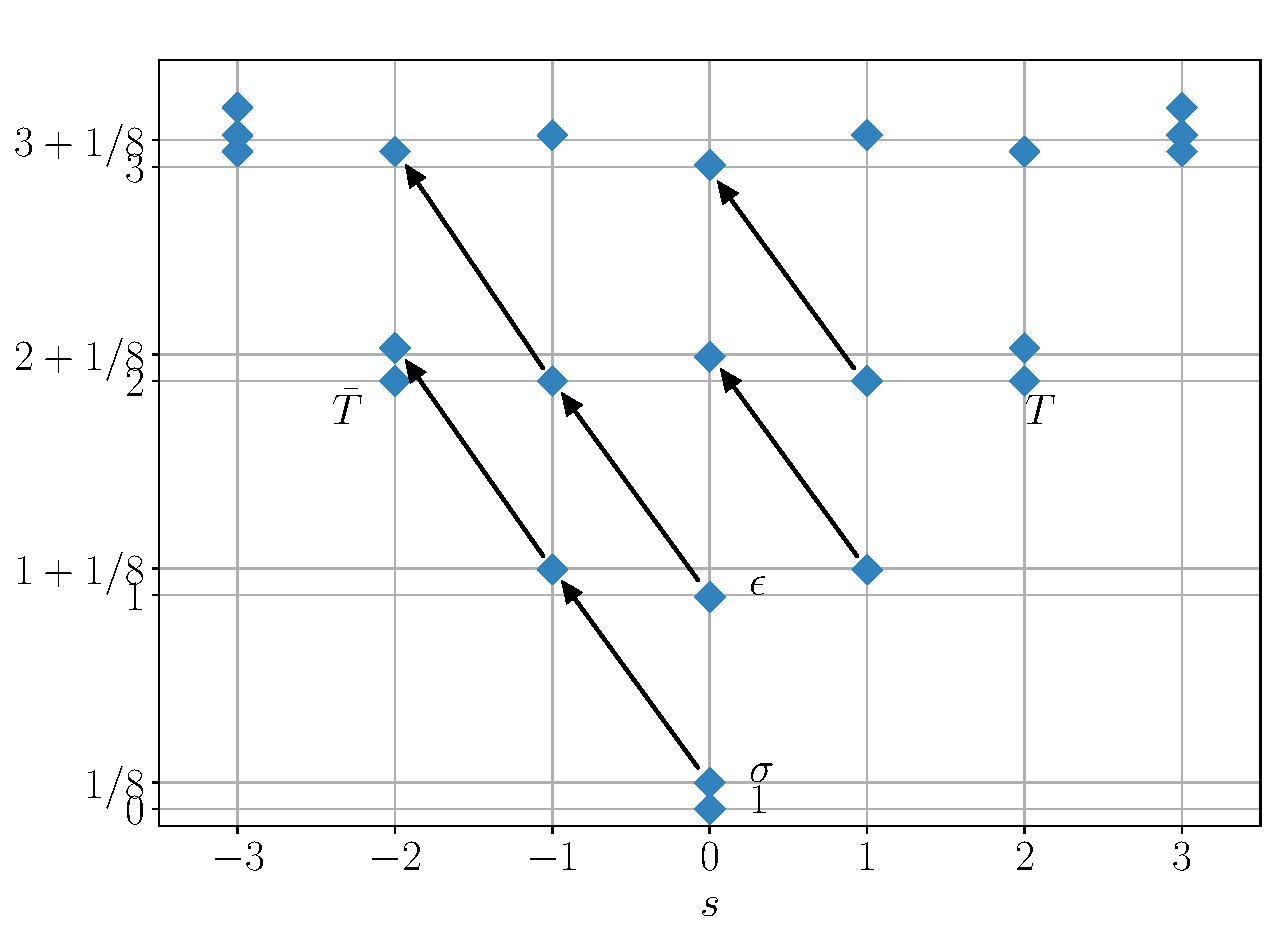
\includegraphics[width=0.42\textwidth]{images/virasoro/ising-lbarm1.pdf}} \\
  \subcaptionbox{$      L_{+1}$}{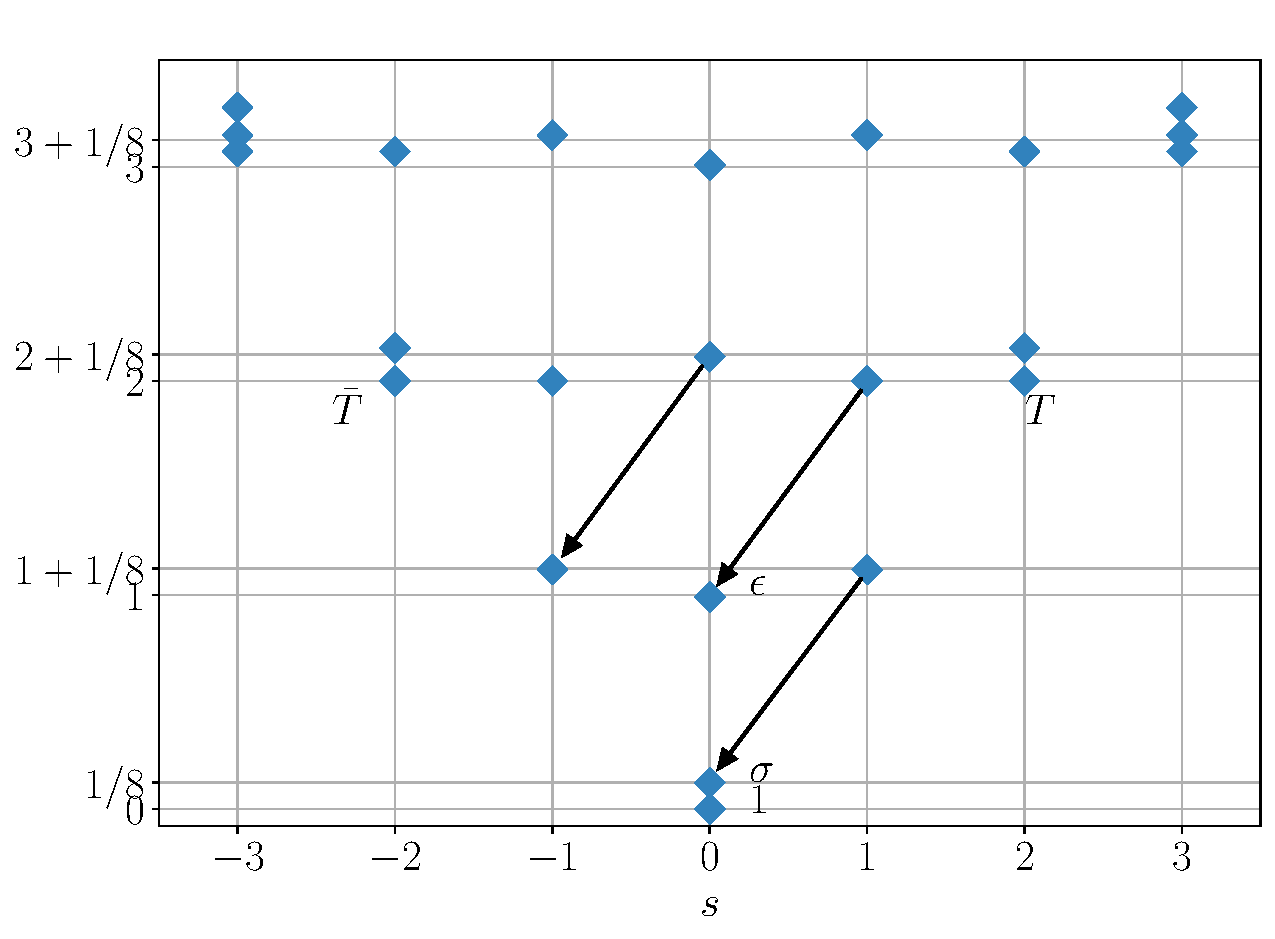
\includegraphics[width=0.42\textwidth]{images/virasoro/ising-l1.pdf}}     \qquad
  \subcaptionbox{$\bar{L}_{+1}$}{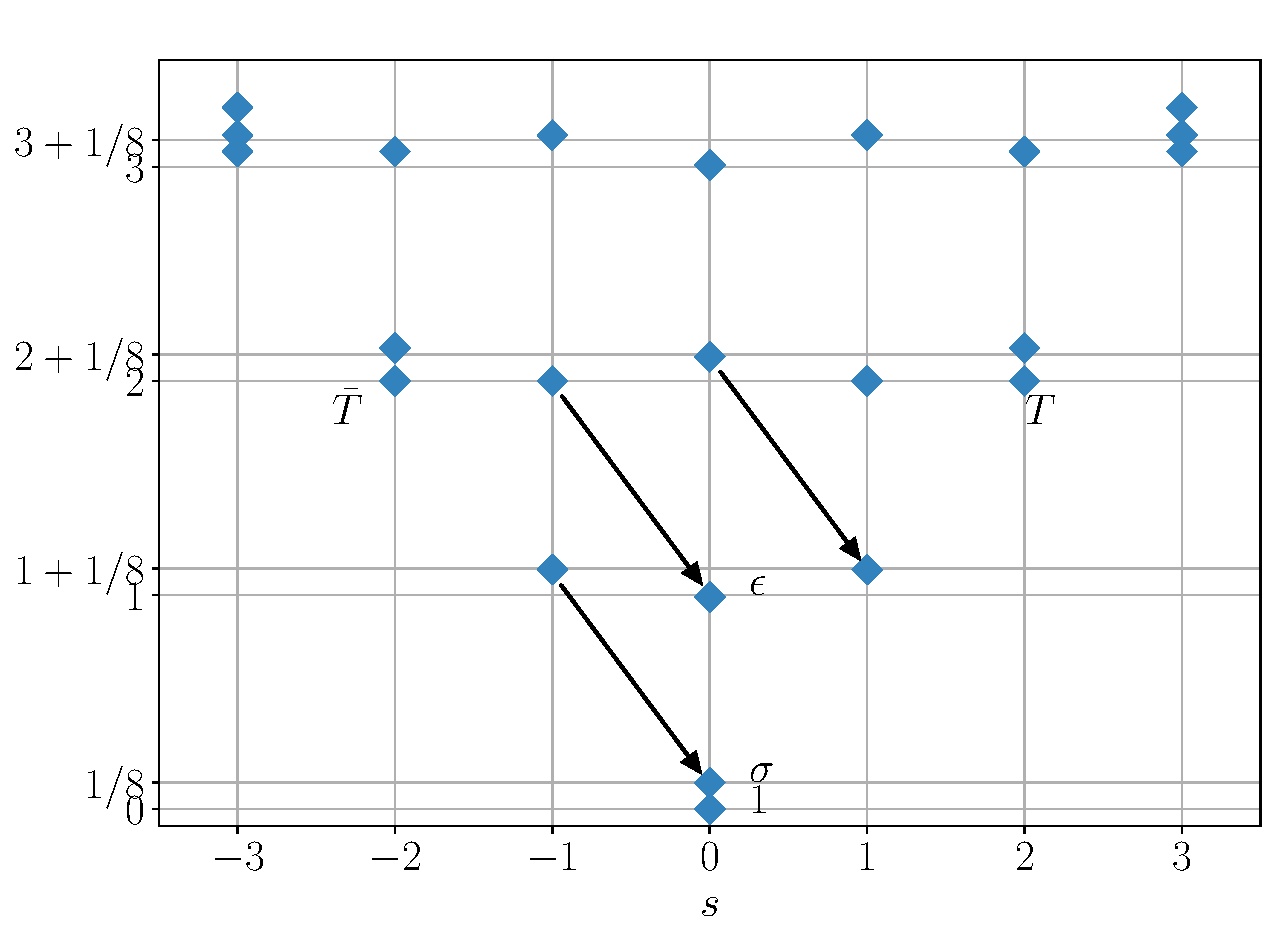
\includegraphics[width=0.42\textwidth]{images/virasoro/ising-lbar1.pdf}}  \\
  \subcaptionbox{$      L_{-2}$}{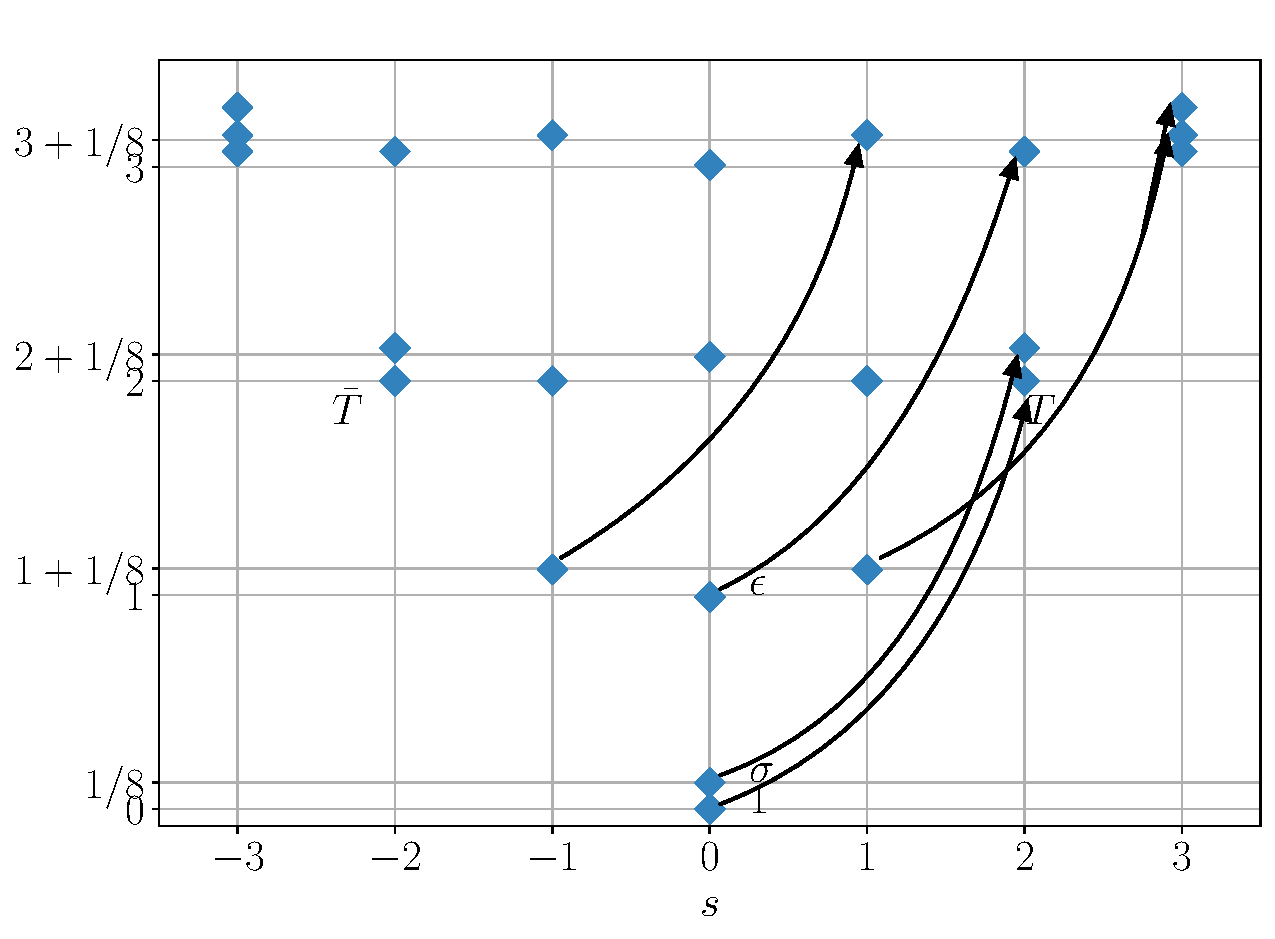
\includegraphics[width=0.42\textwidth]{images/virasoro/ising-lm2.pdf}}    \qquad
  \subcaptionbox{$\bar{L}_{-2}$}{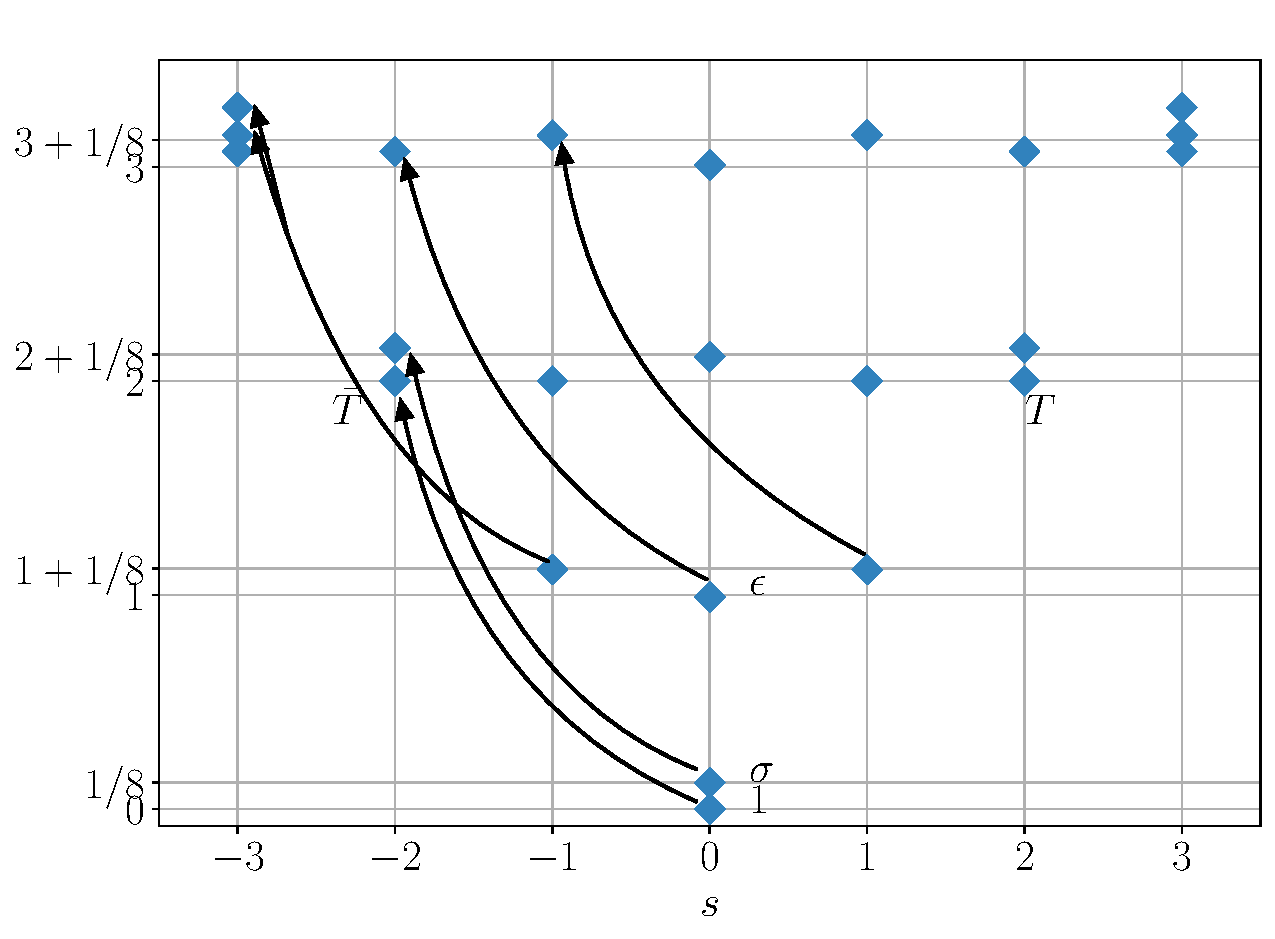
\includegraphics[width=0.42\textwidth]{images/virasoro/ising-lbarm2.pdf}} \\
  \subcaptionbox{$      L_{+2}$}{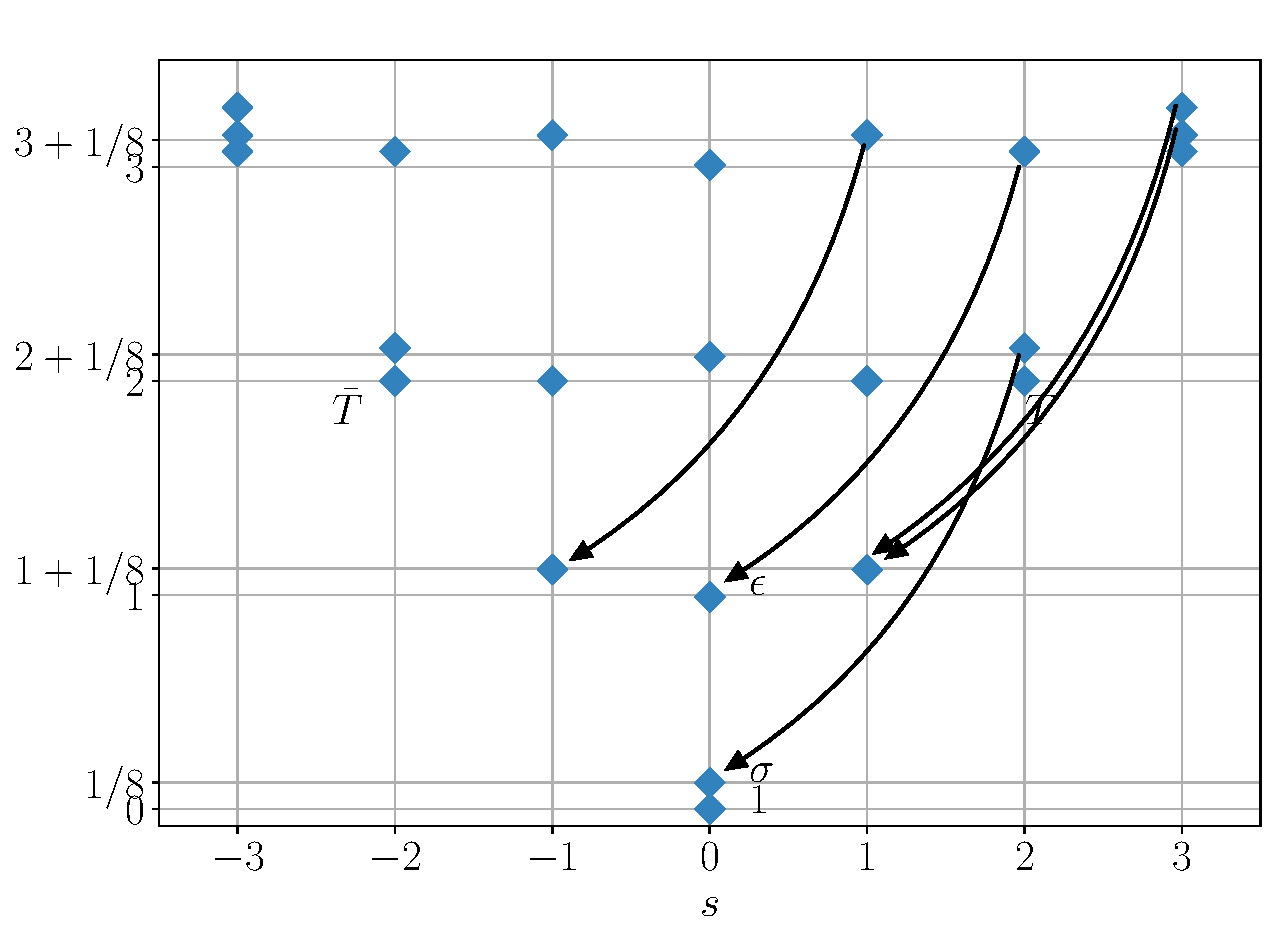
\includegraphics[width=0.42\textwidth]{images/virasoro/ising-l2.pdf}}     \qquad
  \subcaptionbox{$\bar{L}_{+2}$}{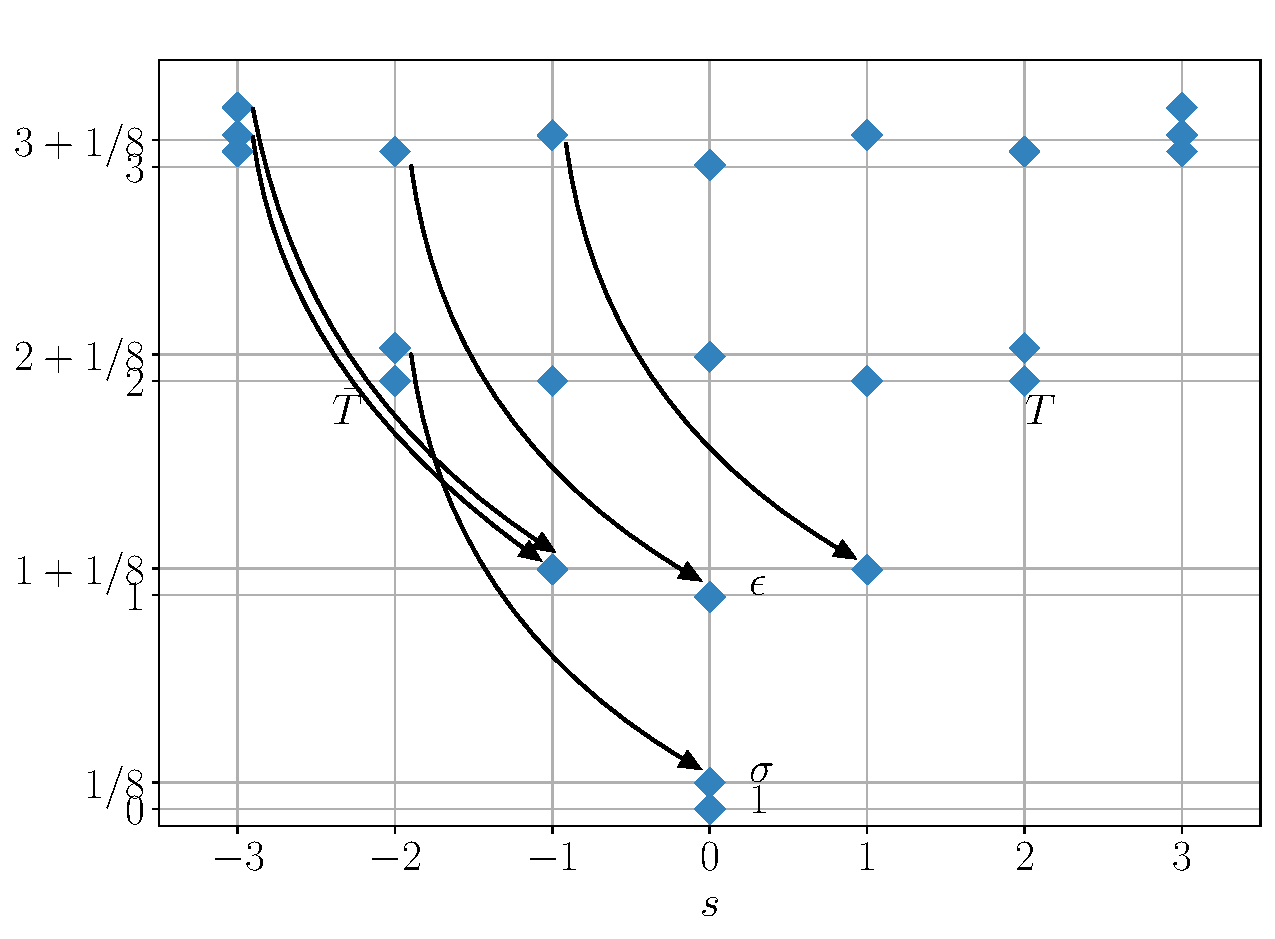
\includegraphics[width=0.42\textwidth]{images/virasoro/ising-lbar2.pdf}}
  \caption[Virasoro 算符在 Ising 模型能谱上的作用]{Virasoro 算符在 Ising 模型能谱上的作用。图片来源:\parencite{wang2022virasoro}。}
  \vspace*{-1.5cm}
  \label{fig:ising-virasoro-all}
\end{figure}

\begin{figure}[ht]
  \centering
  \subcaptionbox{$      J_{-1}$}{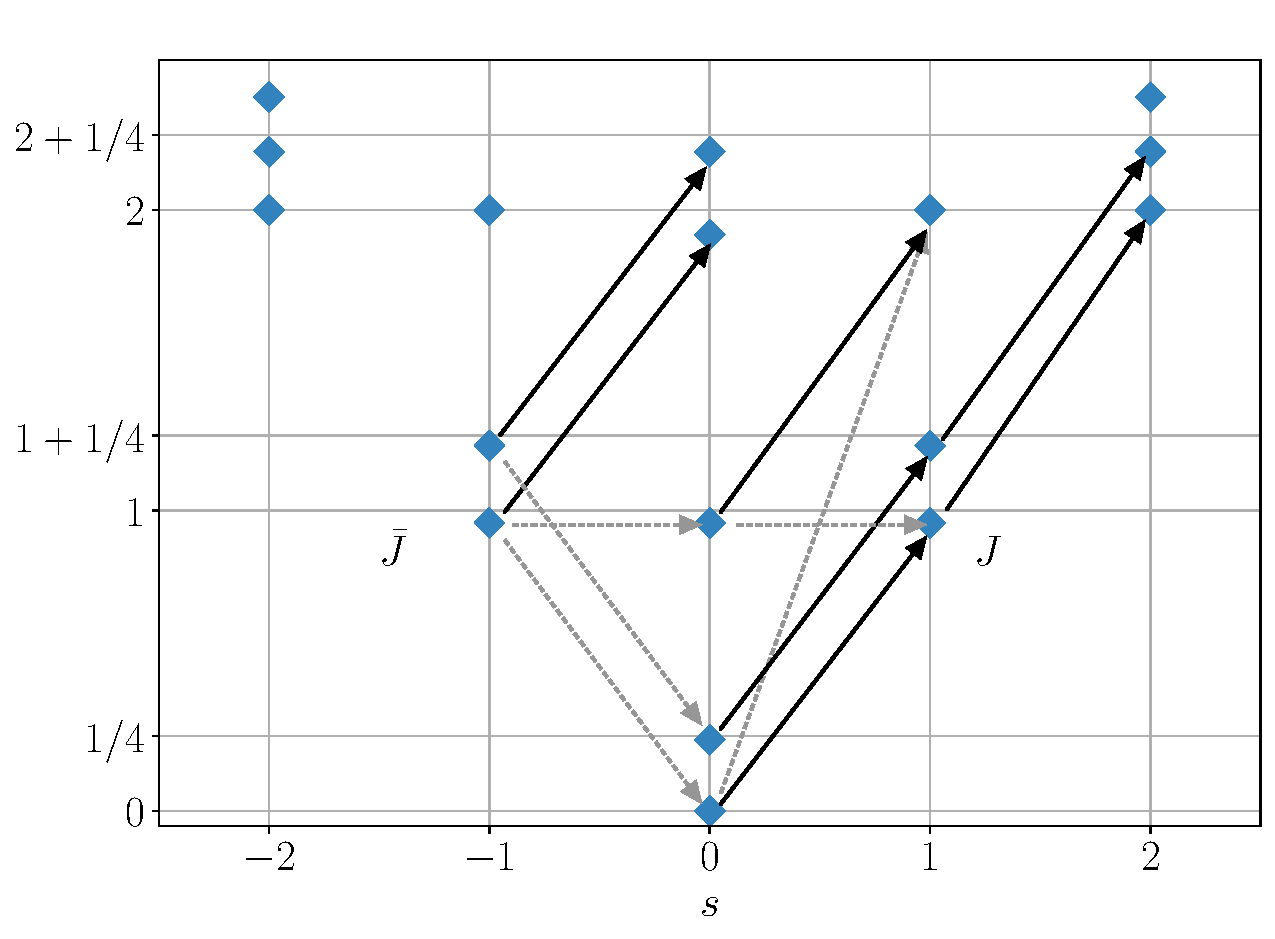
\includegraphics[width=0.42\textwidth]{images/virasoro/dimer-jm1.pdf}}    \qquad
  \subcaptionbox{$\bar{J}_{-1}$}{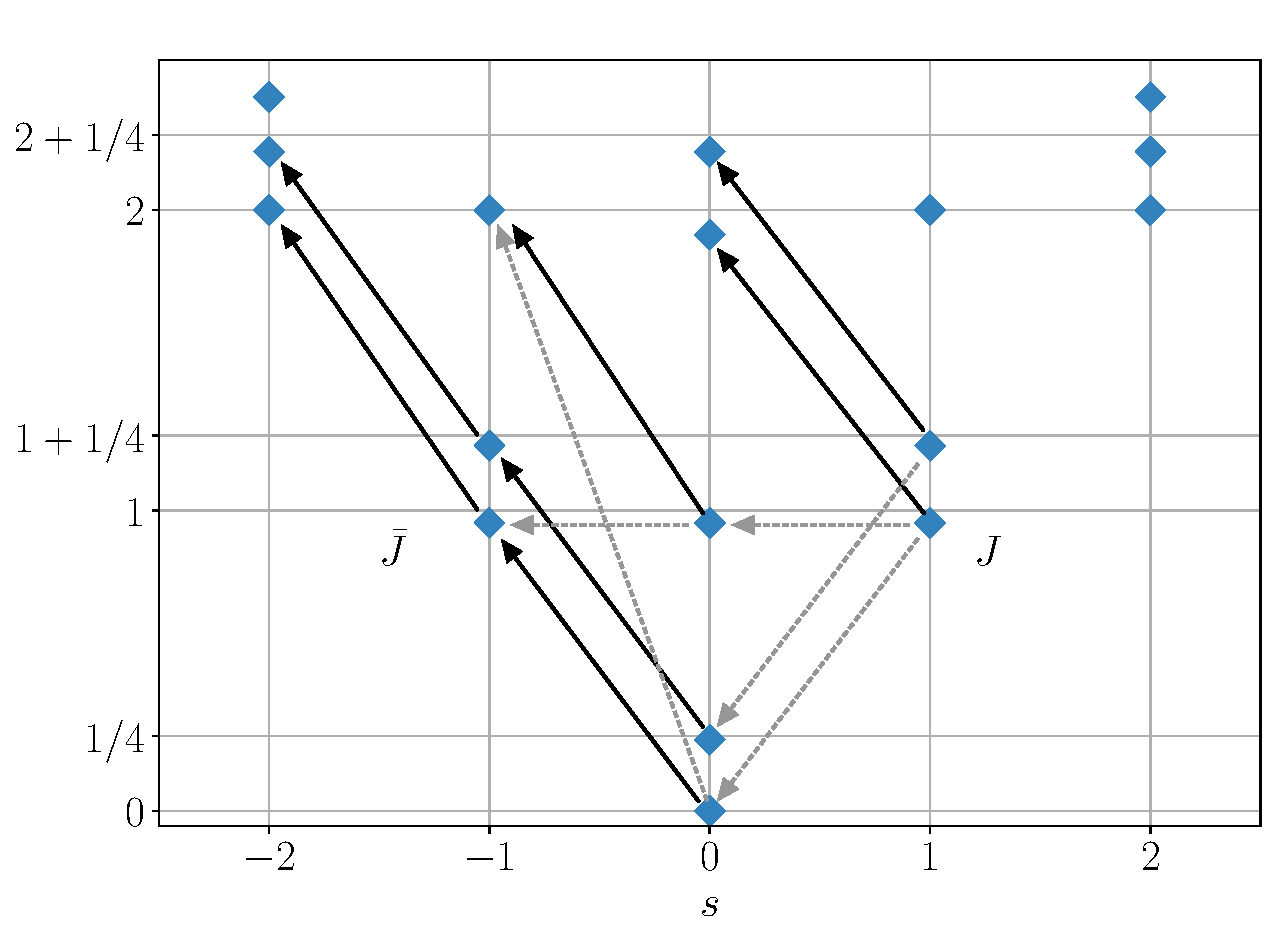
\includegraphics[width=0.42\textwidth]{images/virasoro/dimer-jbarm1.pdf}} \\
  \subcaptionbox{$      J_{-2}$}{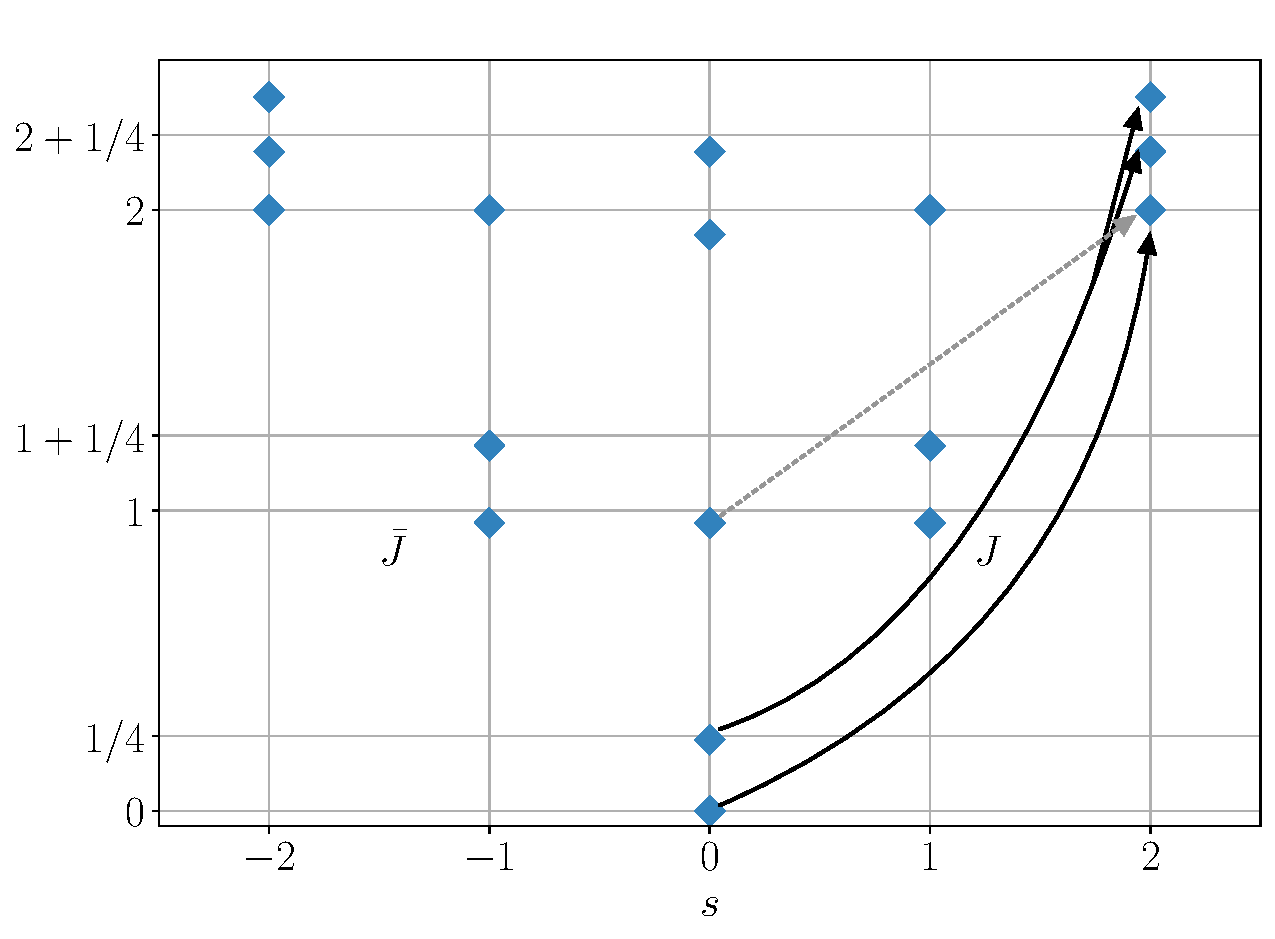
\includegraphics[width=0.42\textwidth]{images/virasoro/dimer-jm2.pdf}}    \qquad
  \subcaptionbox{$\bar{J}_{-2}$}{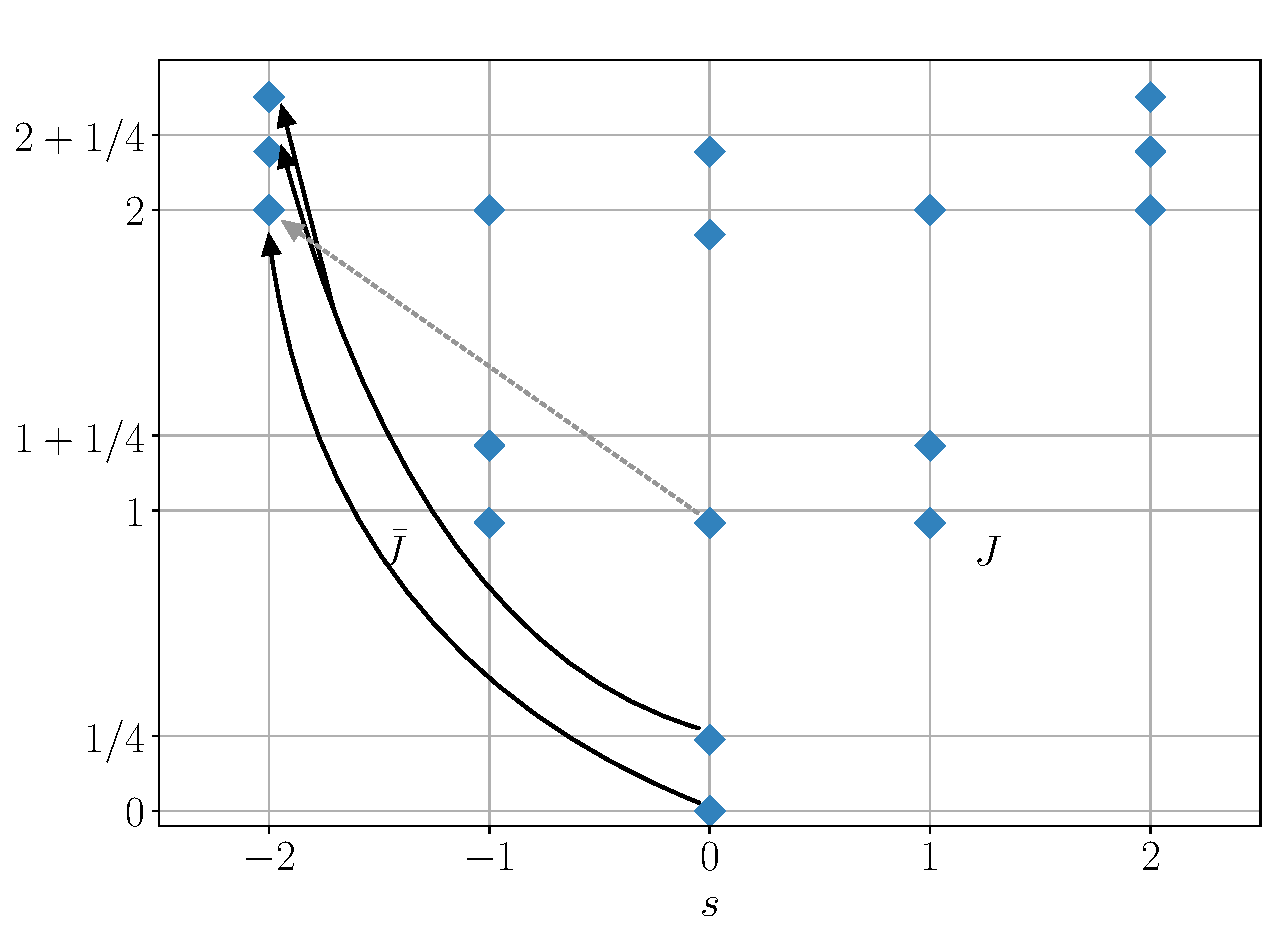
\includegraphics[width=0.42\textwidth]{images/virasoro/dimer-jbarm2.pdf}}
  \caption[Kac--Moody 算符在 dimer 模型能谱上的作用]{Kac--Moody 算符在 dimer 模型能谱上的作用。图片来源:\parencite{wang2022virasoro}。}
  \label{fig:dimer-kac-moody-all}
\end{figure}

\begin{figure}[ht]
  \centering
  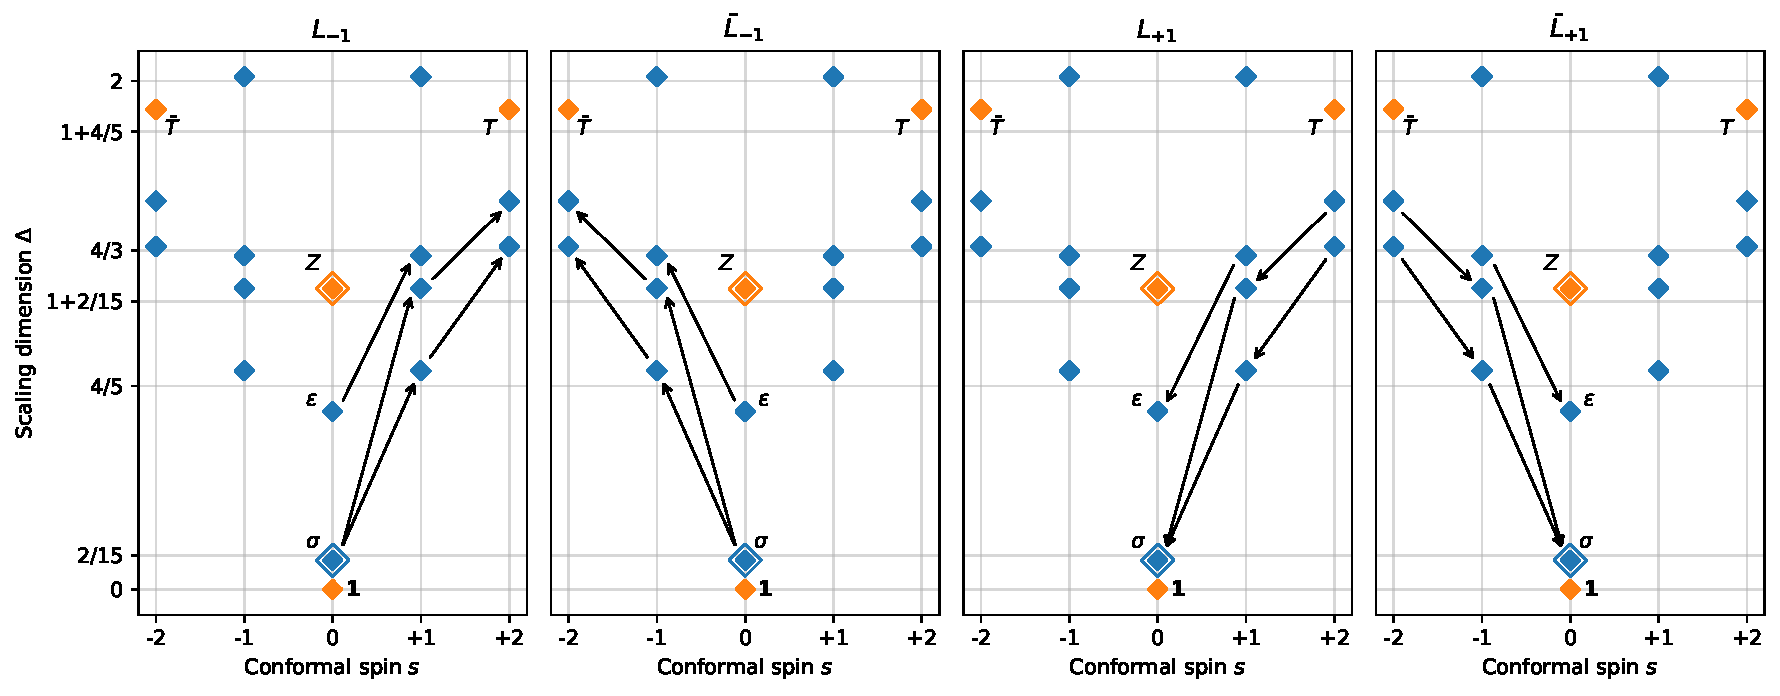
\includegraphics[width=\textwidth]{images/fibonacci/fib-virasoro-all-1.pdf} \\
  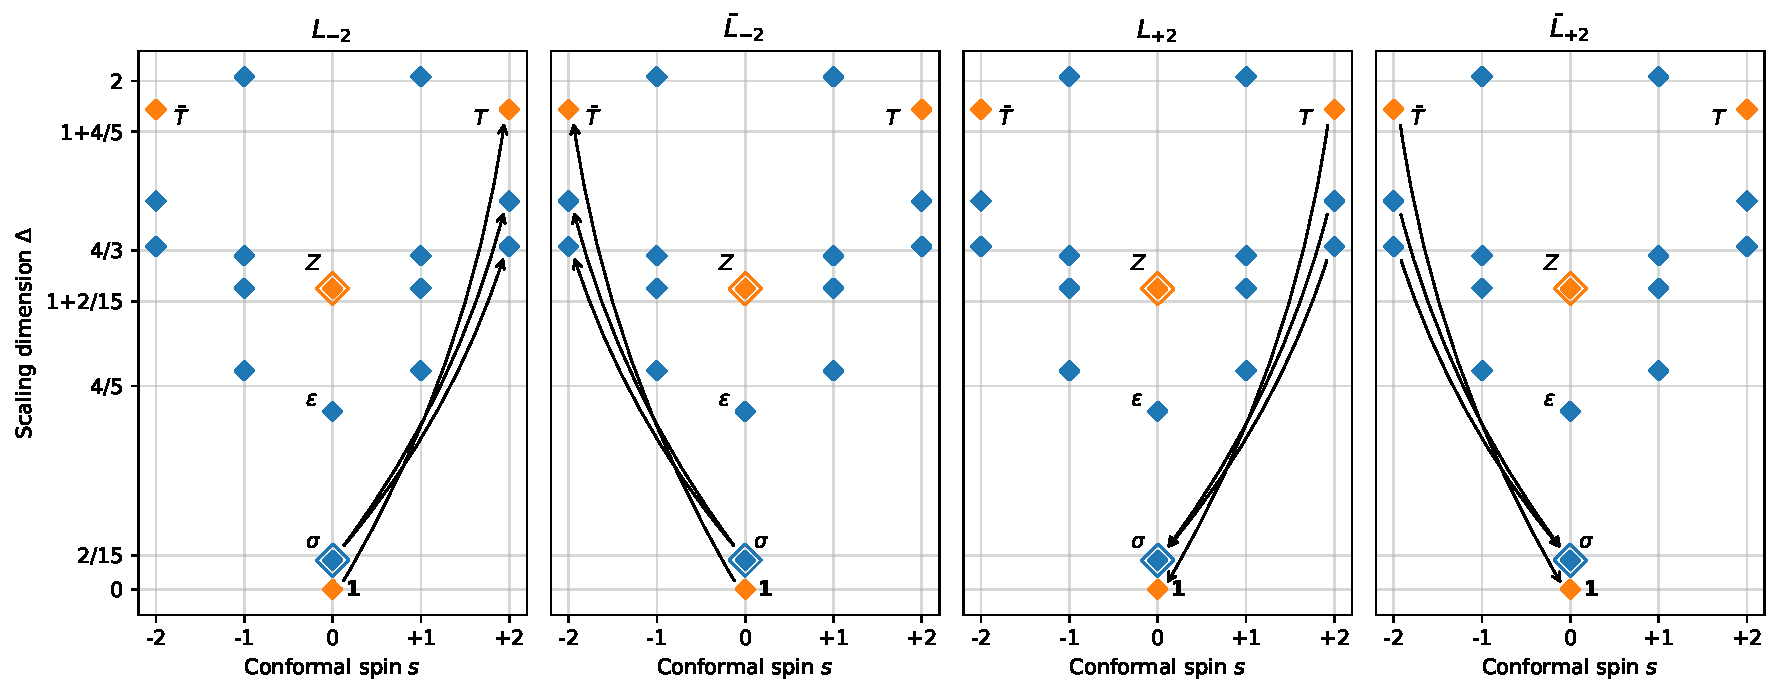
\includegraphics[width=\textwidth]{images/fibonacci/fib-virasoro-all-2.pdf}
  \caption[Virasoro 算符在 Fibonacci 模型能谱上的作用]{Virasoro 算符在 Fibonacci 模型能谱上的作用。图片来源:\parencite{zeng2023virasoro}。}
  \label{fig:fib-virasoro-all}
\end{figure}

\begin{sidewaystable}[ht]
  % \special{pdf: put @thispage <</Rotate 90>>}
  \centering
  \renewcommand{\arraystretch}{1}
  \begin{tabular}{*{8}{c}>{\addfontfeatures{Fractions=On}}c}
    \toprule
      \diagbox{自旋}{标度维数}{圆柱尺寸}
                  & 4        & 8        & 12       & 16       & 20       & 24       & $\infty$     & 理论值 \\
    \midrule
      0           & 0.123499 & 0.124606 & 0.124823 & 0.124900 & 0.124936 & 0.124955 & 0.12522\,(6) & 1/8   \\
      0           & 1.026740 & 1.006488 & 1.002868 & 1.001610 & 1.001030 & 1.000715 & 0.9961\,(11) & 1     \\
      $\pm1$      & 1.245699 & 1.151345 & 1.136446 & 1.131388 & 1.129074 & 1.127824 & 1.107\,(5)   & 1+1/8 \\
      $\pm1,\pm2$ & 2.569513 & 2.098365 & 2.041544 & 2.022974 & 2.014590 & 2.010090 & 1.916\,(30)  & 2     \\
      0           & 2.367899 & 2.178085 & 2.148069 & 2.137876 & 2.133212 & 2.130692 & 2.089\,(11)  & 2+1/8 \\
      $\pm2$      & -        & 2.369005 & 2.223018 & 2.178379 & 2.158670 & 2.148201 & 2.043\,(19)  & 2+1/8 \\
    \bottomrule
  \end{tabular}
  \caption[Ising 模型的能谱数据]{Ising 模型的能谱数据。圆柱(转移矩阵)的尺寸 $n$ 由 4 取到 24,并且外推至无穷大。注意此处 $\Delta_\alpha$ 没有根据 $\Delta_T=2$ 的性质来进行标定。}
  \label{tab:ising-spectrum}
\end{sidewaystable}

\begin{sidewaystable}[ht]
  % \special{pdf: put @thispage <</Rotate 270>>}
  \centering
  \renewcommand{\arraystretch}{1}
  \begin{threeparttable}
    \catcode`\"=\active
    \def"#1"{\textbf{#1}}
    \def\TPTtagStyle#1{\textit{#1}}
    \begin{tabular}{*{10}{c}>{\addfontfeatures{Fractions=On}}c}
      \toprule
        \diagbox{自旋}{标度\\[-0.5ex]维数}{圆柱\\[-0.5ex]尺寸}
                     &  9                  &  12        &  15        &  18        &  21        &  24        &  27        &  $\infty$     &  调整值       &  理论值 \\
      \midrule
        "0"          & "0.0"               & "0.0"      & "0.0"      & "0.0"      & "0.0"      & "0.0"      & "0.0"      & "0.0"         & "0.0"         & "0"     \\
         0\tnote{a}  &  0.112899           &  0.113952  &  0.114474  &  0.114769  &  0.114950  &  0.115070  &  0.115152  &  0.11610\,(7) &  0.1513\,(32) &  2/15   \\
         0           &  0.722756           &  0.709100  &  0.703083  &  0.699890  &  0.697989  &  0.696765  &  0.695931  &  0.6856\,(9)  &  0.894\,(19)  &  4/5    \\
         $\pm1$      &  0.785553           &  0.817591  &  0.841528  &  0.859630  &  0.873686  &  0.884880  &  0.893989  &  0.9557\,(27) &  1.246\,(27)  &  1+2/15 \\
         $\pm1$      &  1.594955           &  1.346025  &  1.242196  &  1.184631  &  1.147942  &  1.122492  &  1.103796  &  0.914\,(11)  &  1.191\,(29)  &  1+2/15 \\
        "0"\tnote{a} & "1.290074"          & "1.222673" & "1.196184" & "1.182805" & "1.175050" & "1.170137" & "1.166820" & "1.123\,(4)"  & "1.464\,(32)" & "4/3"   \\
         $\pm1$      &  1.147427           &  1.222649  &  1.274342  &  1.312081  &  1.340887  &  1.363620  &  1.382029  &  1.510\,(4)   &  1.97\,(4)    &  1+4/5  \\
         $\pm1$      &  3.221770           &  2.490495  &  2.169235  &  2.016147  &  1.925379  &  1.865017  &  1.821876  &  1.31\,(5)    &  1.70\,(8)    &  1+4/5  \\
        "\textpm2"   & "2.727358"\tnote{b} & "2.139950" & "1.967143" & "1.887302" & "1.842910" & "1.815429" & "1.797149" & "1.535\,(33)" & "2.00\,(6)"   & "2"     \\
         $\pm2$      &  1.032723\tnote{b}  &  1.178227  &  1.276463  &  1.348394  &  1.403716  &  1.447739  &  1.483672  &  1.730\,(9)   &  2.25\,(5)    &  2+2/15 \\
         $\pm2$      &  -\tnote{b}         &  1.430687  &  1.484488  &  1.527193  &  1.561317  &  1.589035  &  1.611935  &  1.759\,(9)   &  2.29\,(5)    &  2+2/15 \\
      \bottomrule
    \end{tabular}
    \begin{tablenotes}
      \item[a] 这些能级带有二重简并。
      \item[b] 对于 $n=9$ 的情况,转移矩阵不够大,因此一些高能级的后代没有出现;同时,自旋 $\pm2$ 会退化为 $\pm1$。
    \end{tablenotes}
    \caption[Fibonacci 模型的能谱数据]{Fibonacci 模型的能谱数据。真空态及其后代(标记为粗体)通过对角化带有幂等元的转移矩阵确定,见 \ref{subsec:topological-projectors} 小节。$n=\infty$ 处的数据通过对尺寸由 12 到 27 的圆柱(转移矩阵)本征值外推得到。}
    \label{tab:fib-spectrum}
  \end{threeparttable}
\end{sidewaystable}

\cleardoublepage

在 \ref{subsec:operator-pushing-fib} 小节中,2+1 维 Fibonacci 模型的通解由式~\eqref{eq:2+1d-fib-null-space} 中向量 $v^{(p)}$ 的线性组合与特解部分 $A^{(\mu)}$ 共同组成,且分别对应不同的 $B=\sigma_\mu$。这些 $A^{(\mu)}$ 是 $8\times8$ 的矩阵,它们的最后 3 列均为零,即
\begin{equation}
  A^{(\mu)} = \begin{pmatrix}
    \tilde{A}^{(\mu)} & \mathbf{0} & \mathbf{0} & \mathbf{0}
  \end{pmatrix}.
  \label{eq:2+1d-fib-solution-1}
\end{equation}
这里 $8\times5$ 的矩阵 $\tilde{A}^{(\mu)}$ 由下式给出,其中 $\phi=(1+\sqrt5)/2$,$\omega=\ee^{\ii\pi/5}$:
\begingroup
\small
\allowdisplaybreaks
\begin{align}
  \tilde{A}^{(0)} &= \begin{pmatrix}
    1 & 0 & 0 & 0 & 0 \\
    0 & 1 & 0 & 0 & 0 \\
    0 & 0 & 1 & 0 & 0 \\
    0 & 0 & 0 & 1 & 0 \\
    0 & 0 & 0 & 0 & 1 \\
    0 & 0 & 1 & 1 & -1 \\
    0 & 1 & 0 & 1 & -1 \\
    \phi & \sqrt{\phi} & \sqrt{\phi} & -\frac{1}{\sqrt{\phi}} & \frac{\phi+1}{\sqrt{\phi}} \\
  \end{pmatrix}, &
  \tilde{A}^{(1)} &= \begin{pmatrix}
    0 & 0 & 0 & 0 & \frac{1}{\phi} \\
    0 & 0 & 1 & 0 & 0 \\
    0 & 0 & 0 & \frac{1}{\sqrt{\phi}} & -\frac{1}{\sqrt{\phi}} \\
    \phi^{3/2} & 1 & 0 & 0 & 0 \\
    0 & 1 & 0 & 0 & 0 \\
    \phi^{3/2} & 0 & 0 & \frac{1}{\sqrt{\phi}} & -\frac{1}{\sqrt{\phi}} \\
    \phi^{3/2} & 0 & 1 & 0 & 0 \\
    -\phi & \sqrt{\phi} & \sqrt{\phi} & 1 & 0 \\
  \end{pmatrix}, \notag \\[2ex]
  %
  \tilde{A}^{(2)} &= \begin{pmatrix}
    0 & \frac{1}{\phi} & 0 & 0 & 0 \\
    0 & 0 & 0 & \frac{1}{\sqrt{\phi}} & -\frac{1}{\sqrt{\phi}} \\
    \phi & 0 & 0 & 0 & 0 \\
    0 & 0 & 1 & 0 & \sqrt{\phi} \\
    0 & 0 & 1 & 0 & 0 \\
    \phi & 0 & 0 & 0 & \sqrt{\phi} \\
    0 & 0 & 0 & \frac{1}{\sqrt{\phi}} & \frac{\phi-1}{\sqrt{\phi}} \\
    \phi^{3/2} & 1 & \sqrt{\phi} & 1 & -2 \\
  \end{pmatrix}, &
  \tilde{A}^{(3)} &= \begin{pmatrix}
    0 & 0 & \frac{1}{\phi} & 0 & 0 \\
    \phi & 0 & 0 & 0 & 0 \\
    0 & 0 & 0 & 0 & 1 \\
    0 & \sqrt{\phi} & 0 & \frac{1}{\sqrt{\phi}} & -\frac{1}{\sqrt{\phi}} \\
    0 & 0 & 0 & \frac{1}{\sqrt{\phi}} & -\frac{1}{\sqrt{\phi}} \\
    0 & \sqrt{\phi} & 0 & 0 & 1 \\
    \phi & \sqrt{\phi} & 0 & 0 & 0 \\
    \phi^{3/2} & -1 & 1 & 1 & \sqrt{\phi}-1 \\
  \end{pmatrix}, \notag \\[2ex]
  %
  \tilde{A}^{(4)} &= \begin{pmatrix}
    0 & 0 & 0 & \frac{1}{\phi^{3/2}} & -\frac{1}{\phi^{3/2}} \\
    0 & 0 & 0 & 0 & 1 \\
    0 & 1 & 0 & 0 & 0 \\
    \phi & 0 & \sqrt{\phi} & 0 & 0 \\
    \phi & 0 & 0 & 0 & 0 \\
    0 & 1 & \sqrt{\phi} & 0 & 0 \\
    0 & 0 & \sqrt{\phi} & 0 & 1 \\
    \phi^{3/2} & \sqrt{\phi} & -1 & \frac{1}{\sqrt{\phi}} & \frac{\phi-1}{\sqrt{\phi}} \\
  \end{pmatrix}, &
  \tilde{A}^{(5)} &= \begin{pmatrix}
    1 & 0 & 0 & 0 & 0 \\
    0 & \omega^4 & 0 & 0 & 0 \\
    0 & 0 & -\omega & 0 & 0 \\
    0 & 0 & 0 & -\omega^3 & \omega^3+\omega^2 \\
    0 & 0 & 0 & 0 & \omega^2 \\
    0 & 0 & -\omega & -\omega^3 & \omega^3 \\
    0 & \omega^4 & 0 & -\omega^3 & \omega^3 \\
    \phi & \omega^4 \sqrt{\phi} & -\omega\sqrt{\phi} & \frac{\omega^3}{\sqrt{\phi}} & \frac{\omega^2 \phi-\omega^3}{\sqrt{\phi}} \\
  \end{pmatrix}, \notag \\[2ex]
  %
  \tilde{A}^{(6)} &= \begin{pmatrix}
    0 & 0 & 0 & 0 & \frac{\omega^2}{\phi} \\
    0 & 0 & -\omega & 0 & 0 \\
    0 & 0 & 0 & -\frac{\omega^3}{\sqrt{\phi}} & \frac{\omega^3}{\sqrt{\phi}} \\
    \phi^{3/2} & \omega^4 & 0 & 0 & 0 \\
    0 & \omega^4 & 0 & 0 & 0 \\
    \phi^{3/2} & 0 & 0 & -\frac{\omega^3}{\sqrt{\phi}} & \frac{\omega^3}{\sqrt{\phi}} \\
    \phi^{3/2} & 0 & -\omega & 0 & 0 \\
    -\phi & \omega^4 \sqrt{\phi} & -\omega\sqrt{\phi} & -\omega^3 & \omega^3+\omega^2 \\
  \end{pmatrix}, &
  \tilde{A}^{(7)} &= \begin{pmatrix}
    0 & \frac{\omega^4}{\phi} & 0 & 0 & 0 \\
    0 & 0 & 0 & -\frac{\omega^3}{\sqrt{\phi}} & \frac{\omega^3}{\sqrt{\phi}} \\
    \phi & 0 & 0 & 0 & 0 \\
    0 & 0 & -\omega & 0 & \omega^2 \sqrt{\phi} \\
    0 & 0 & -\omega & 0 & 0 \\
    \phi & 0 & 0 & 0 & \omega^2 \sqrt{\phi} \\
    0 & 0 & 0 & -\frac{\omega^3}{\sqrt{\phi}} & \frac{\omega^3+\omega^2 \phi}{\sqrt{\phi}} \\
    \phi^{3/2} & \omega^4 & -\omega\sqrt{\phi} & -\omega^3 & \omega^3-\omega^2 \\
  \end{pmatrix}, \notag \\[2ex]
  %
  \tilde{A}^{(8)} &= \begin{pmatrix}
    0 & 0 & -\frac{\omega}{\phi} & 0 & 0 \\
    \phi & 0 & 0 & 0 & 0 \\
    0 & 0 & 0 & 0 & \omega^2 \\
    0 & \omega^4 \sqrt{\phi} & 0 & -\frac{\omega^3}{\sqrt{\phi}} & \frac{\omega^3}{\sqrt{\phi}} \\
    0 & 0 & 0 & -\frac{\omega^3}{\sqrt{\phi}} & \frac{\omega^3}{\sqrt{\phi}} \\
    0 & \omega^4 \sqrt{\phi} & 0 & 0 & \omega^2 \\
    \phi & \omega^4 \sqrt{\phi} & 0 & 0 & 0 \\
    \phi^{3/2} & -\omega^4 & -\omega & -\omega^3 & \omega^3+\omega^2 \sqrt{\phi} \\
  \end{pmatrix}, &
  \tilde{A}^{(9)} &= \begin{pmatrix}
    0 & 0 & 0 & -\frac{\omega^3}{\phi^{3/2}} & \frac{\omega^3}{\phi^{3/2}} \\
    0 & 0 & 0 & 0 & \omega^2 \\
    0 & \omega^4 & 0 & 0 & 0 \\
    \phi & 0 & -\omega\sqrt{\phi} & 0 & 0 \\
    \phi & 0 & 0 & 0 & 0 \\
    0 & \omega^4 & -\omega\sqrt{\phi} & 0 & 0 \\
    0 & 0 & -\omega\sqrt{\phi} & 0 & \omega^2 \\
    \phi^{3/2} & \omega^4 \sqrt{\phi} & \omega & -\frac{\omega^3}{\sqrt{\phi}} & \frac{\omega^3+\omega^2 \phi}{\sqrt{\phi}} \\
  \end{pmatrix}, \notag \\[2ex]
  %
  \tilde{A}^{(10)} &= \begin{pmatrix}
    1 & 0 & 0 & 0 & 0 \\
    0 & -\omega^3 & 0 & 0 & 0 \\
    0 & 0 & \omega^2 & 0 & 0 \\
    0 & 0 & 0 & -\omega & \omega^4+\omega \\
    0 & 0 & 0 & 0 & \omega^4 \\
    0 & 0 & \omega^2 & -\omega & \omega \\
    0 & -\omega^3 & 0 & -\omega & \omega \\
    \phi & -\omega^3\sqrt{\phi} & \omega^2 \sqrt{\phi} & \frac{\omega}{\sqrt{\phi}} & \frac{\omega^4 \phi-\omega}{\sqrt{\phi}} \\
  \end{pmatrix}, &
  \tilde{A}^{(11)} &= \begin{pmatrix}
    0 & 0 & 0 & 0 & \frac{\omega^4}{\phi} \\
    0 & 0 & \omega^2 & 0 & 0 \\
    0 & 0 & 0 & -\frac{\omega}{\sqrt{\phi}} & \frac{\omega}{\sqrt{\phi}} \\
    \phi^{3/2} & -\omega^3 & 0 & 0 & 0 \\
    0 & -\omega^3 & 0 & 0 & 0 \\
    \phi^{3/2} & 0 & 0 & -\frac{\omega}{\sqrt{\phi}} & \frac{\omega}{\sqrt{\phi}} \\
    \phi^{3/2} & 0 & \omega^2 & 0 & 0 \\
    -\phi & -\omega^3\sqrt{\phi} & \omega^2 \sqrt{\phi} & -\omega & \omega^4+\omega \\
  \end{pmatrix}, \notag \\[2ex]
  %
  \tilde{A}^{(12)} &= \begin{pmatrix}
    0 & -\frac{\omega^3}{\phi} & 0 & 0 & 0 \\
    0 & 0 & 0 & -\frac{\omega}{\sqrt{\phi}} & \frac{\omega}{\sqrt{\phi}} \\
    \phi & 0 & 0 & 0 & 0 \\
    0 & 0 & \omega^2 & 0 & \omega^4 \sqrt{\phi} \\
    0 & 0 & \omega^2 & 0 & 0 \\
    \phi & 0 & 0 & 0 & \omega^4 \sqrt{\phi} \\
    0 & 0 & 0 & -\frac{\omega}{\sqrt{\phi}} & \frac{\omega+\omega^4 \phi}{\sqrt{\phi}} \\
    \phi^{3/2} & -\omega^3 & \omega^2 \sqrt{\phi} & -\omega & \omega-\omega^4 \\
  \end{pmatrix}, &
  \tilde{A}^{(13)} &= \begin{pmatrix}
    0 & 0 & \frac{\omega^2}{\phi} & 0 & 0 \\
    \phi & 0 & 0 & 0 & 0 \\
    0 & 0 & 0 & 0 & \omega^4 \\
    0 & -\omega^3\sqrt{\phi} & 0 & -\frac{\omega}{\sqrt{\phi}} & \frac{\omega}{\sqrt{\phi}} \\
    0 & 0 & 0 & -\frac{\omega}{\sqrt{\phi}} & \frac{\omega}{\sqrt{\phi}} \\
    0 & -\omega^3\sqrt{\phi} & 0 & 0 & \omega^4 \\
    \phi & -\omega^3\sqrt{\phi} & 0 & 0 & 0 \\
    \phi^{3/2} & \omega^3 & \omega^2 & -\omega & \omega+\omega^4 \sqrt{\phi} \\
  \end{pmatrix}, \notag \\[2ex]
  %
  \tilde{A}^{(14)} &= \begin{pmatrix}
    0 & 0 & 0 & -\frac{\omega}{\phi^{3/2}} & \frac{\omega}{\phi^{3/2}} \\
    0 & 0 & 0 & 0 & \omega^4 \\
    0 & -\omega^3 & 0 & 0 & 0 \\
    \phi & 0 & \omega^2 \sqrt{\phi} & 0 & 0 \\
    \phi & 0 & 0 & 0 & 0 \\
    0 & -\omega^3 & \omega^2 \sqrt{\phi} & 0 & 0 \\
    0 & 0 & \omega^2 \sqrt{\phi} & 0 & \omega^4 \\
    \phi^{3/2} & -\omega^3\sqrt{\phi} & -\omega^2 & -\frac{\omega}{\sqrt{\phi}} & \frac{\omega+\omega^4 \phi}{\sqrt{\phi}} \\
  \end{pmatrix}, &
  \tilde{A}^{(15)} &= \begin{pmatrix}
    1 & 0 & 0 & 0 & 0 \\
    0 & \omega^2 & 0 & 0 & 0 \\
    0 & 0 & -\omega^3 & 0 & 0 \\
    0 & 0 & 0 & \omega^4 & -\omega^4-\omega \\
    0 & 0 & 0 & 0 & -\omega \\
    0 & 0 & -\omega^3 & \omega^4 & -\omega^4 \\
    0 & \omega^2 & 0 & \omega^4 & -\omega^4 \\
    \phi & \omega^2 \sqrt{\phi} & -\omega^3\sqrt{\phi} & -\frac{\omega^4}{\sqrt{\phi}} & \frac{\omega^4-\omega \phi}{\sqrt{\phi}} \\
  \end{pmatrix}, \notag \\[2ex]
  %
  \tilde{A}^{(16)} &= \begin{pmatrix}
    0 & 0 & 0 & 0 & -\frac{\omega}{\phi} \\
    0 & 0 & -\omega^3 & 0 & 0 \\
    0 & 0 & 0 & \frac{\omega^4}{\sqrt{\phi}} & -\frac{\omega^4}{\sqrt{\phi}} \\
    \phi^{3/2} & \omega^2 & 0 & 0 & 0 \\
    0 & \omega^2 & 0 & 0 & 0 \\
    \phi^{3/2} & 0 & 0 & \frac{\omega^4}{\sqrt{\phi}} & -\frac{\omega^4}{\sqrt{\phi}} \\
    \phi^{3/2} & 0 & -\omega^3 & 0 & 0 \\
    -\phi & \omega^2 \sqrt{\phi} & -\omega^3\sqrt{\phi} & \omega^4 & -\omega^4-\omega \\
  \end{pmatrix}, &
  \tilde{A}^{(17)} &= \begin{pmatrix}
    0 & \frac{\omega^2}{\phi} & 0 & 0 & 0 \\
    0 & 0 & 0 & \frac{\omega^4}{\sqrt{\phi}} & -\frac{\omega^4}{\sqrt{\phi}} \\
    \phi & 0 & 0 & 0 & 0 \\
    0 & 0 & -\omega^3 & 0 & -\omega\sqrt{\phi} \\
    0 & 0 & -\omega^3 & 0 & 0 \\
    \phi & 0 & 0 & 0 & -\omega\sqrt{\phi} \\
    0 & 0 & 0 & \frac{\omega^4}{\sqrt{\phi}} & \frac{-\omega^4-\omega \phi}{\sqrt{\phi}} \\
    \phi^{3/2} & \omega^2 & -\omega^3\sqrt{\phi} & \omega^4 & \omega-\omega^4 \\
  \end{pmatrix}, \notag \\[2ex]
  %
  \tilde{A}^{(18)} &= \begin{pmatrix}
    0 & 0 & -\frac{\omega^3}{\phi} & 0 & 0 \\
    \phi & 0 & 0 & 0 & 0 \\
    0 & 0 & 0 & 0 & -\omega \\
    0 & \omega^2 \sqrt{\phi} & 0 & \frac{\omega^4}{\sqrt{\phi}} & -\frac{\omega^4}{\sqrt{\phi}} \\
    0 & 0 & 0 & \frac{\omega^4}{\sqrt{\phi}} & -\frac{\omega^4}{\sqrt{\phi}} \\
    0 & \omega^2 \sqrt{\phi} & 0 & 0 & -\omega \\
    \phi & \omega^2 \sqrt{\phi} & 0 & 0 & 0 \\
    \phi^{3/2} & -\omega^2 & -\omega^3 & \omega^4 & -\omega^4-\omega \sqrt{\phi} \\
  \end{pmatrix}, &
  \tilde{A}^{(19)} &= \begin{pmatrix}
    0 & 0 & 0 & \frac{\omega^4}{\phi^{3/2}} & -\frac{\omega^4}{\phi^{3/2}} \\
    0 & 0 & 0 & 0 & -\omega \\
    0 & \omega^2 & 0 & 0 & 0 \\
    \phi & 0 & -\omega^3\sqrt{\phi} & 0 & 0 \\
    \phi & 0 & 0 & 0 & 0 \\
    0 & \omega^2 & -\omega^3\sqrt{\phi} & 0 & 0 \\
    0 & 0 & -\omega^3\sqrt{\phi} & 0 & -\omega \\
    \phi^{3/2} & \omega^2 \sqrt{\phi} & \omega^3 & \frac{\omega^4}{\sqrt{\phi}} & \frac{-\omega^4-\omega \phi}{\sqrt{\phi}} \\
  \end{pmatrix}, \notag \\[2ex]
  %
  \tilde{A}^{(20)} &= \begin{pmatrix}
    1 & 0 & 0 & 0 & 0 \\
    0 & -\omega & 0 & 0 & 0 \\
    0 & 0 & \omega^4 & 0 & 0 \\
    0 & 0 & 0 & \omega^2 & -\omega^3-\omega^2 \\
    0 & 0 & 0 & 0 & -\omega^3 \\
    0 & 0 & \omega^4 & \omega^2 & -\omega^2 \\
    0 & -\omega & 0 & \omega^2 & -\omega^2 \\
    \phi & -\omega\sqrt{\phi} & \omega^4 \sqrt{\phi} & -\frac{\omega^2}{\sqrt{\phi}} & \frac{\omega^2-\omega^3 \phi}{\sqrt{\phi}} \\
  \end{pmatrix}, &
  \tilde{A}^{(21)} &= \begin{pmatrix}
    0 & 0 & 0 & 0 & -\frac{\omega^3}{\phi} \\
    0 & 0 & \omega^4 & 0 & 0 \\
    0 & 0 & 0 & \frac{\omega^2}{\sqrt{\phi}} & -\frac{\omega^2}{\sqrt{\phi}} \\
    \phi^{3/2} & -\omega & 0 & 0 & 0 \\
    0 & -\omega & 0 & 0 & 0 \\
    \phi^{3/2} & 0 & 0 & \frac{\omega^2}{\sqrt{\phi}} & -\frac{\omega^2}{\sqrt{\phi}} \\
    \phi^{3/2} & 0 & \omega^4 & 0 & 0 \\
    -\phi & -\omega\sqrt{\phi} & \omega^4 \sqrt{\phi} & \omega^2 & -\omega^3-\omega^2 \\
  \end{pmatrix}, \notag \\[2ex]
  %
  \tilde{A}^{(22)} &= \begin{pmatrix}
    0 & -\frac{\omega}{\phi} & 0 & 0 & 0 \\
    0 & 0 & 0 & \frac{\omega^2}{\sqrt{\phi}} & -\frac{\omega^2}{\sqrt{\phi}} \\
    \phi & 0 & 0 & 0 & 0 \\
    0 & 0 & \omega^4 & 0 & -\omega^3\sqrt{\phi} \\
    0 & 0 & \omega^4 & 0 & 0 \\
    \phi & 0 & 0 & 0 & -\omega^3\sqrt{\phi} \\
    0 & 0 & 0 & \frac{\omega^2}{\sqrt{\phi}} & \frac{-\omega^3\phi-\omega^2}{\sqrt{\phi}} \\
    \phi^{3/2} & -\omega & \omega^4 \sqrt{\phi} & \omega^2 & \omega^3-\omega^2 \\
  \end{pmatrix}, &
  \tilde{A}^{(23)} &= \begin{pmatrix}
    0 & 0 & \frac{\omega^4}{\phi} & 0 & 0 \\
    \phi & 0 & 0 & 0 & 0 \\
    0 & 0 & 0 & 0 & -\omega^3 \\
    0 & -\omega\sqrt{\phi} & 0 & \frac{\omega^2}{\sqrt{\phi}} & -\frac{\omega^2}{\sqrt{\phi}} \\
    0 & 0 & 0 & \frac{\omega^2}{\sqrt{\phi}} & -\frac{\omega^2}{\sqrt{\phi}} \\
    0 & -\omega\sqrt{\phi} & 0 & 0 & -\omega^3 \\
    \phi & -\omega\sqrt{\phi} & 0 & 0 & 0 \\
    \phi^{3/2} & \omega & \omega^4 & \omega^2 & -\omega^3\sqrt{\phi} -\omega^2 \\
  \end{pmatrix}, \notag \\[2ex]
  %
  \tilde{A}^{(24)} &= \begin{pmatrix}
    0 & 0 & 0 & \frac{\omega^2}{\phi^{3/2}} & -\frac{\omega^2}{\phi^{3/2}} \\
    0 & 0 & 0 & 0 & -\omega^3 \\
    0 & -\omega & 0 & 0 & 0 \\
    \phi & 0 & \omega^4 \sqrt{\phi} & 0 & 0 \\
    \phi & 0 & 0 & 0 & 0 \\
    0 & -\omega & \omega^4 \sqrt{\phi} & 0 & 0 \\
    0 & 0 & \omega^4 \sqrt{\phi} & 0 & -\omega^3 \\
    \phi^{3/2} & -\omega\sqrt{\phi} & -\omega^4 & \frac{\omega^2}{\sqrt{\phi}} & \frac{-\omega^3\phi-\omega^2}{\sqrt{\phi}} \\
  \end{pmatrix}.
  \label{eq:2+1d-fib-solution-2}
\end{align}
\endgroup
